\subsection{General}
\subsubsection{Online TikZ manuel}
\url{https://tikz.dev/}\\
\subsubsection{Package and libraries}
\verb|\usepackage{tikz}| using tikz package\\
\verb|\usetikzlibrary{positioning}| Load a given tikz library\\
\subsubsection{Syntax}
\verb|\coordinate (X) at (3,5);| name a point X\\
\verb|\node[options] (X) at (3,5) {};| place a node and name it X\\

\subsection{Coordinate specifications}
\subsubsection{Coordinate calculations}
\begin{tabular}[]{p{0.1\textwidth}p{0.1\textwidth}l}
&&library needed\\
$(x,y)$&Cartesian coordinates&\\
($\theta$:r)&polar coordinates&\\
\verb |($(A)+{sin(60)}*(B)$)|         &coordinate calculations&calc\\
\verb |($(A)!.25!(B)$)|&                 partway calculations&calc\\
\verb |($(A)!3cm!(B)$)|&                 3~cm from (A) in direction of (B)&calc\\
\verb |($(A)!1.2!30:(B)$)|&              stretch by 1.2, then rotate by 30$^{\circ}$&calc\\
\verb |($(A)!(B)!(C)$)|&                 projection of point B onto line AC&calc\\
\verb |($(A)!(B)!30:(C)$)|&              project B onto line AC, then rotate by 30$^{\circ}$&calc\\
\verb '(n1-|n2)'& projection of n2 on the line passing through n1\\
\verb '(n1|-n2)'& projection of n1 on the line passing through n2\\
\verb |\node[above=1cm of| \verb|somenode.north]|&position new node 1~cm above existing anchor&positioning\\
\end{tabular}
\begin{tikzpicture}
  \node (C) {C}; 
  \node (A) at ($(C)+(120:0.5)$) {A};
  \node (B) at ($(C)+(240:0.5)$) {B};
  \node (D) at ($(C)+(360:0.5)$) {D};
  \draw (C) -- (A);
  \draw (C) -- (B);
  \draw (C) -- (D);
\end{tikzpicture}
\begin{minipage}[c]{3cm}
  \begin{verbatim}
\begin{tikzpicture}
  \node (C) {C}; 
  \node (A) at ($(C)+(120:0.5)$) {A};
  \node (B) at ($(C)+(240:0.5)$) {B};
  \node (D) at ($(C)+(360:0.5)$) {D};
  \draw (C) -- (A);
  \draw (C) -- (B);
  \draw (C) -- (D);
\end{tikzpicture}
  \end{verbatim}
\end{minipage}\\
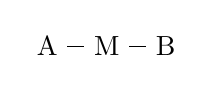
\begin{tikzpicture}
  \node (A) {A};
  \node[right=of A] (B) {B};
  \path (A) -- (B) node[midway] (M) {M};
  \draw (A) -- (M) -- (B);
\end{tikzpicture}
\begin{minipage}[c]{3cm}
  \begin{verbatim}
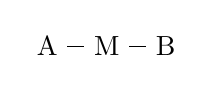
\begin{tikzpicture}
  \node (A) {A};
  \node[right=of A] (B) {B};
  \path (A) -- (B) node[midway] (M) {M};
  \draw (A) -- (M) -- (B);
\end{tikzpicture}
  \end{verbatim}
\end{minipage}\\

\subsubsection{Absolute positioning on the page}
\begin{verbatim}
\begin{tikzpicture}[remember picture, overlay]
  \node [] (node1) at (current page.west) {};
\end{tikzpicture}
\end{verbatim}
\includegraphics[width=0.33\textwidth]{figures/rectangle_shape.pdf}
\subsubsection{Matrix positioning}
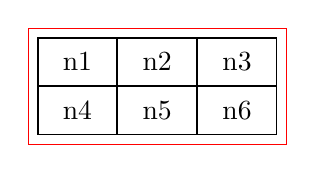
\begin{tikzpicture}
  [n/.style={draw,minimum width=1cm,minimum height=4ex,color=black}]
  \matrix[draw,color=red] (M) {
    \node[n] {n1}; &&
    \node[n] {n2}; &&
    \node[n] {n3}; \\
    \node[n] {n4}; &&
    \node[n] {n5}; &&
    \node[n] {n6}; \\
  };
\end{tikzpicture}
\begin{minipage}[c]{3cm}
  \begin{verbatim}
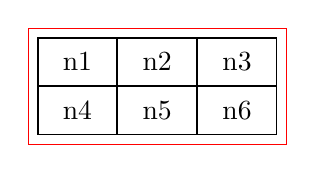
\begin{tikzpicture}
  [n/.style={draw,
             minimum width=1cm,
             minimum height=4ex,
             color=black}]
  \matrix[draw,color=red] (M) {
    \node[n] {n1}; &&
    \node[n] {n2}; &&
    \node[n] {n3}; \\
    \node[n] {n4}; &&
    \node[n] {n5}; &&
    \node[n] {n6}; \\
  };
\end{tikzpicture}
  \end{verbatim}
\end{minipage}

\subsection{Node dimension}
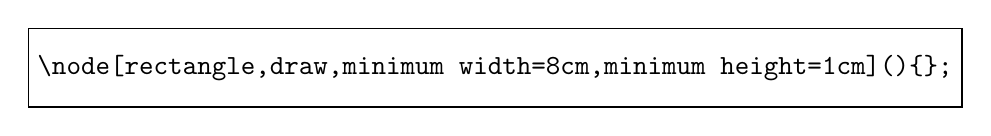
\begin{tikzpicture}
\node[rectangle,draw,minimum width=8cm, minimum height=1cm] () {\verb|\node[rectangle,draw,minimum width=8cm,minimum height=1cm](){};|};
\end{tikzpicture}

\subsection{Node shapes and filling colors}

\begin{tikzpicture}
  \node[rectangle,draw=black,minimum width=1.5cm, minimum height=4ex] (rectangle) {}; 
  \node[right=0.2cm of rectangle]{\verb|\node[rectangle,draw=black](){};|};
\end{tikzpicture}

\begin{tikzpicture}
  \node[rectangle,draw=black,minimum width=1.5cm, minimum height=4ex,rounded corners] (rectangle) {}; 
  \node[right=0.2cm of rectangle]{\verb|\node[rectangle,draw=black,rounded corners](){};|};
\end{tikzpicture}

\begin{tikzpicture}
  \node[rectangle,draw=black,minimum width=1.5cm, minimum height=4ex,fill=blue] (rectangle) {}; 
  \node[right=0.2cm of rectangle]{\verb|\node[rectangle,draw=black,fill=blue](){};|};
\end{tikzpicture}

\subsection{Node options}
\subsubsection{Fonts and text colors}
\verb |node font=\tiny|\\
\verb |font=\bfseries| Node font in bold\\
\verb |text=blue| text color\\
\subsubsection{Text alignment in nodes}
\verb 'align=left|center|right' (handling carriage return in nodes)\\
\subsubsection{Style definition}
\verb |\begin{tikzpicture}[stylename/.style={node options...}]| Defining a node style named stylename\\
\verb |node[stylename] (node1) {};| Using a defined style

\subsection{Arrows}
\begin{verbatim}
\coordinate (P1);
\coordinate[right=of P1] (P2);
\end{verbatim}
\begin{tikzpicture}
  \coordinate (P1);
  \coordinate[right=of P1] (P2);
  \draw[->] (P1) -- (P2);
  \node[right of=P2, anchor=west] {\verb|\draw[->] (P1) -- (P2);|};
\end{tikzpicture}
\begin{tikzpicture}
  \coordinate (P1);
  \coordinate[right=of P1] (P2);
  \draw[-Stealth] (P1) -- (P2);
  \node[right of=P2, anchor=west] {\verb|\draw[-Stealth] (P1) -- (P2);|};
\end{tikzpicture}
\begin{tikzpicture}
  \coordinate (P1);
  \coordinate[right=of P1] (P2);
  \draw[-{Stealth[round]}] (P1) -- (P2);
  \node[right of=P2, anchor=west] {\verb|\draw[-{Stealth[round]}] (P1) -- (P2);|};
\end{tikzpicture}
\begin{tikzpicture}
  \coordinate (P1);
  \coordinate[right=of P1] (P2);
  \draw[-{Stealth[round,length=4mm]}] (P1) -- (P2);
  \node[right of=P2, anchor=west] {\verb|\draw[-{Stealth[round,length=4mm]}] (P1) -- (P2);|};
\end{tikzpicture}
\verb |\begin{tikzpicture}[>={Stealth[round]}]| Defining an arrow style for the whole picture\\
